\documentclass[10pt,a4paper,oneside,twocolumn]{article}

    \usepackage{float}	% for floating figures (putting them anywhere we want
    \usepackage{amsmath}	% for maths
    \usepackage{graphicx}	% jpg
    \usepackage{hyperref}
    \usepackage{textcomp}
    \usepackage{verbatim}	% use of \begin{comment}
    \usepackage{pgfplots}	% use of pgf plots
    \usepackage{multicol}
    \usepackage[top=2cm, bottom=2cm, left=2cm, right=2cm]{geometry} %margins
    \usepackage{sidecap}	% for side captions
    \restylefloat{table}	% floating figures(Tables)
    \usepackage{caption}
    \captionsetup{justification=justified}
    \usepackage{subcaption}

    \numberwithin{equation}{section} %permits numbering within sections instead of globally
\begin{document}

\title{\huge{\textbf{Report}}\\
	\vspace{0.5cm}
	\Large{\textit{\'Ecole Polytechnique F\'ed\'erale de Lausanne, Switzerland}}}
\author{\large{Florian + Dariush}}

\begin{titlepage}
 \maketitle
\thispagestyle{empty}
\end{titlepage}

\section{Introduction}
    Introduction to the article goes here    Introduction to the article goes here  Introduction to the article goes here  Introduction to the article goes here  Introduction to the article goes here  Introduction to the article goes here  Introduction to the article goes here  Introduction to the article goes here  Introduction to the article goes here  Introduction to the article goes here  Introduction to the article goes here  Introduction to the article goes here  Introduction to the article goes here  Introduction to the article goes here  Introduction to the article goes here  Introduction to the article goes here  Introduction to the article goes here  Introduction to the article goes here  Introduction to the article goes here  Introduction to the article goes here  Introduction to the article goes here  Introduction to the article goes here Introduction to the article goes here \\

\section{The Model}

    \begin{figure}[!h]
	\centering
	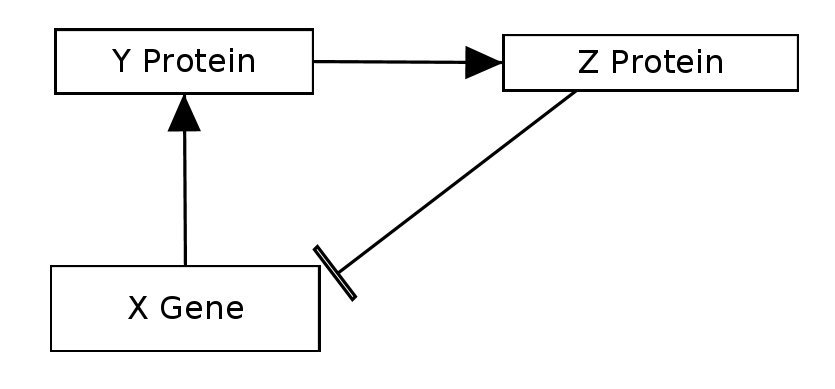
\includegraphics[scale=0.3]{sketch.png}
	\caption{Sketch of that thing blabla}
    \end{figure}
    
    b/ablalaeolauelthaeou

    \begin{figure*}[!h]
	\begin{subfigure}[b]{0.5\textwidth}
	    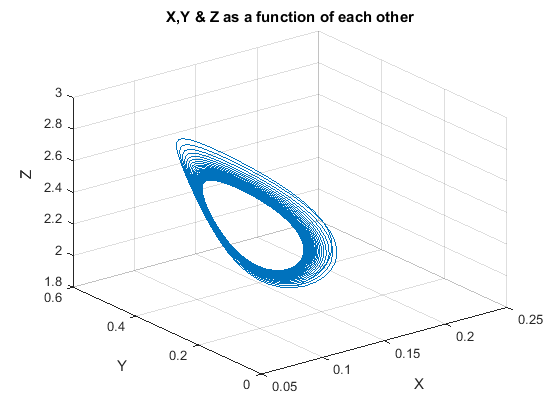
\includegraphics[width=\textwidth]{A11.png}
	    \caption{Trajectories}
	\end{subfigure}
	~
	\begin{subfigure}[b]{0.5\textwidth}
	    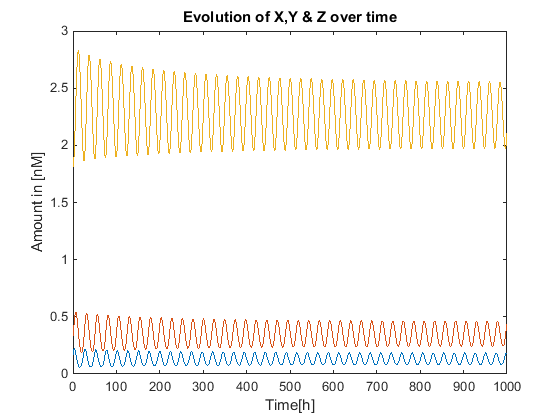
\includegraphics[width=\textwidth]{A12.png}
	    \caption{Frequency spectrum}
	\end{subfigure}
	\caption{With nice initial conditions}
    \end{figure*}

    \begin{figure*}
    \centering
	\begin{subfigure}[b]{0.32\textwidth}
	    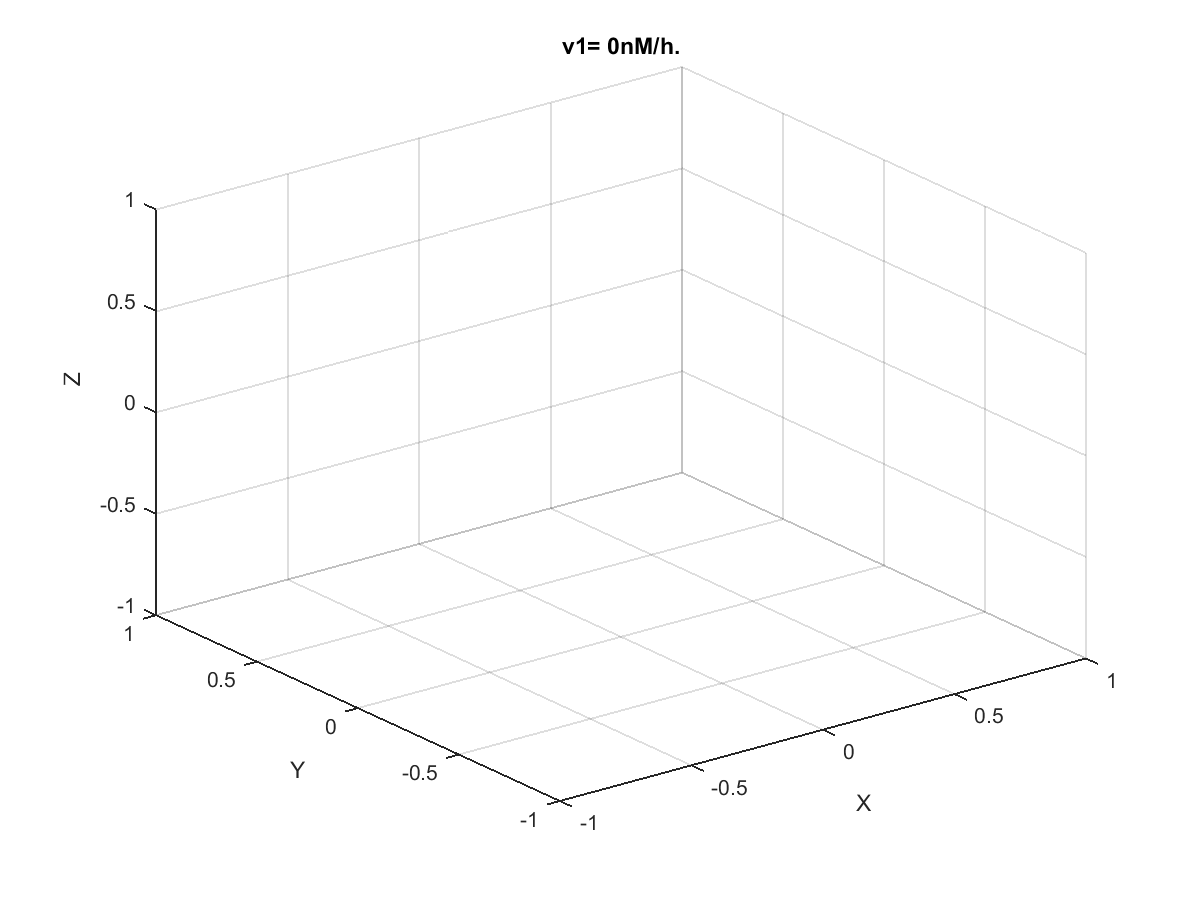
\includegraphics[width=\textwidth]{LotsofthesameA/A-AA0.png}
	    \caption{v1 = 0 nM/h}
	\end{subfigure}
	~ 
	\begin{subfigure}[b]{0.32\textwidth}
	    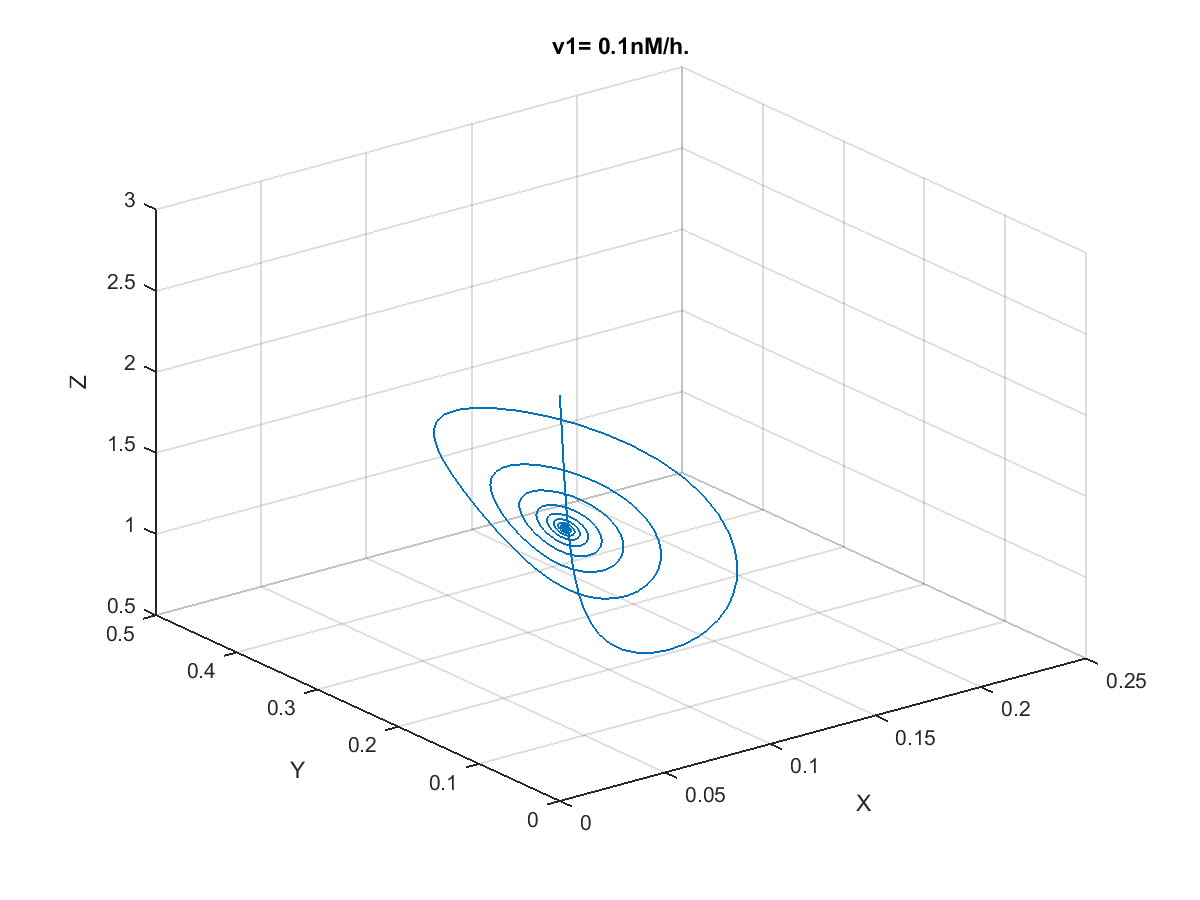
\includegraphics[width=\textwidth]{LotsofthesameA/A-AA1.png}
	    \caption{v1 = 1 nM/h}
	\end{subfigure}
	~ 
	\begin{subfigure}[b]{0.32\textwidth}
	    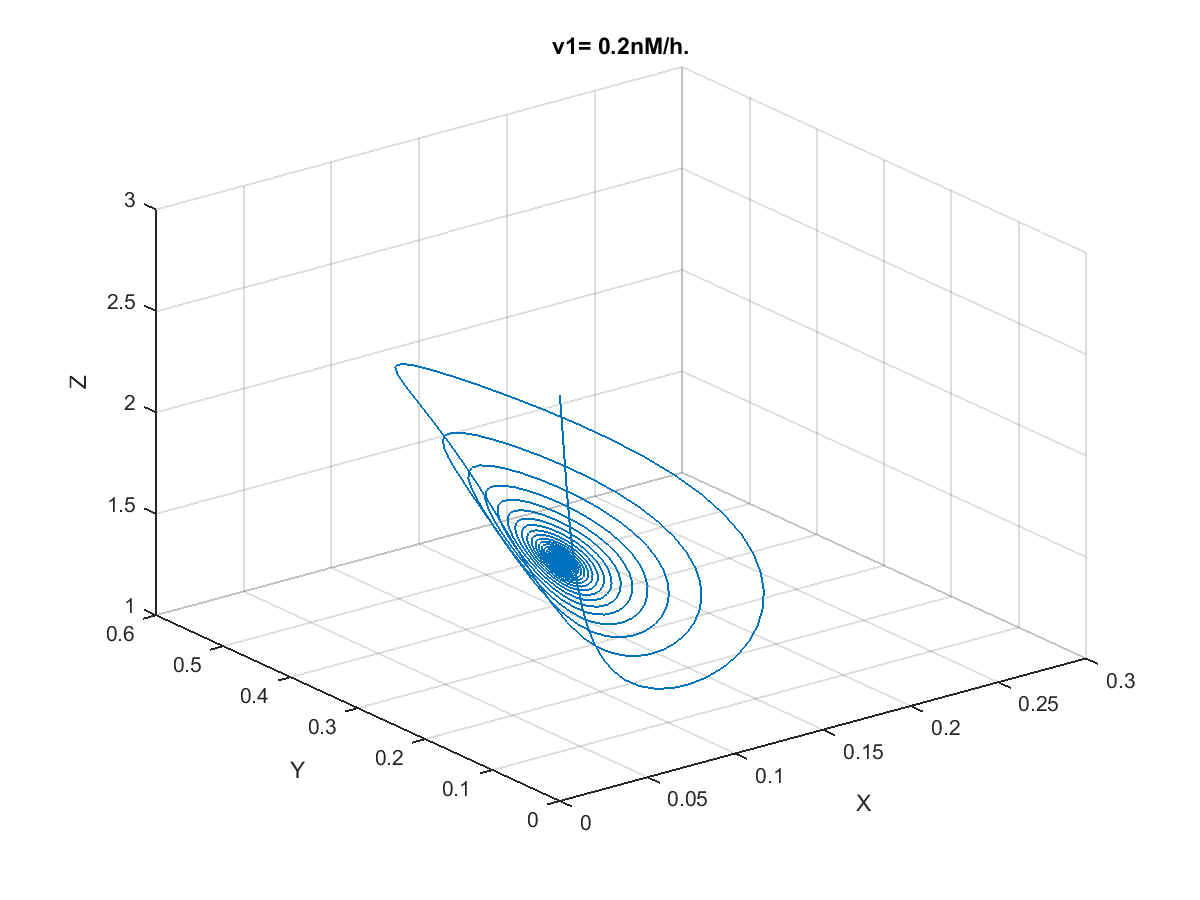
\includegraphics[width=\textwidth]{LotsofthesameA/A-AA2.png}
	    \caption{v1 = 2 nM/h}
	\end{subfigure}
	 
	\begin{subfigure}[b]{0.32\textwidth}
	    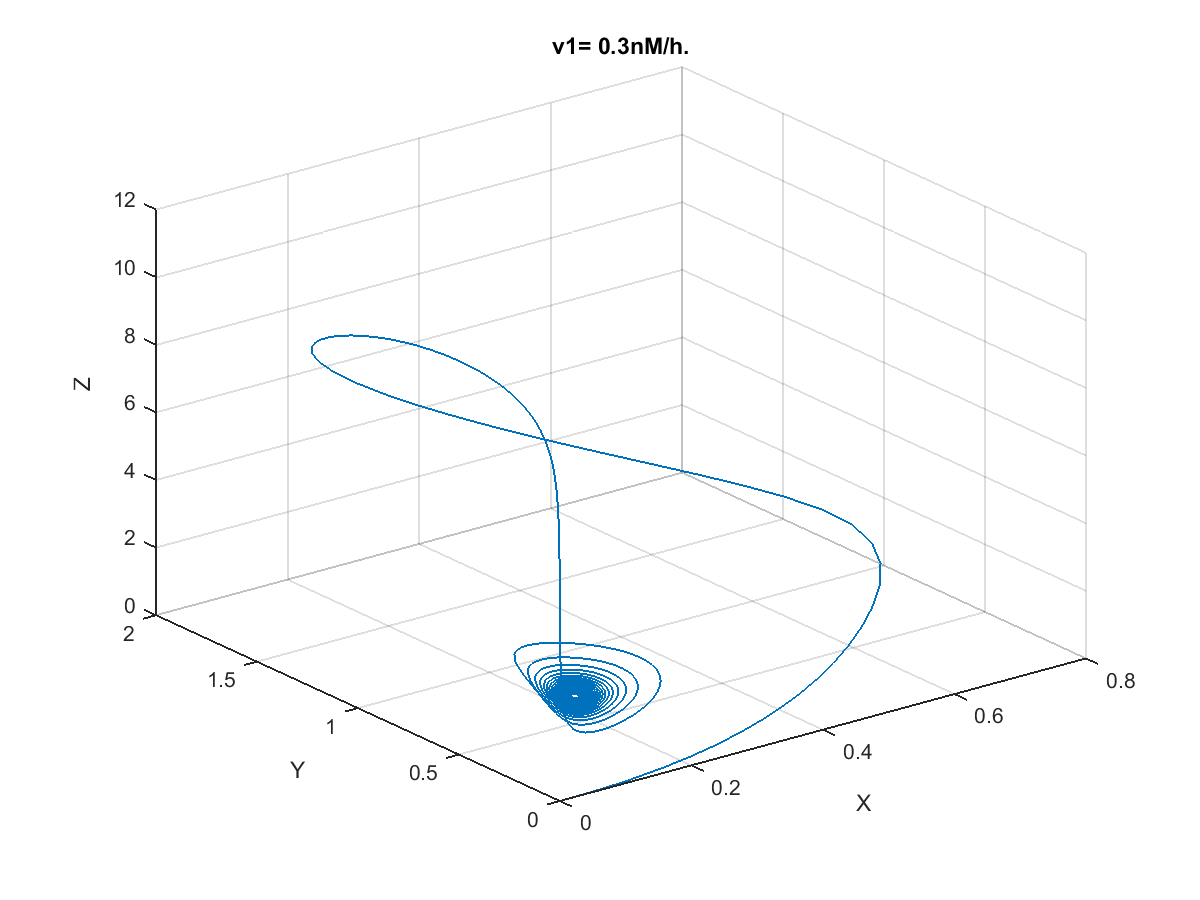
\includegraphics[width=\textwidth]{LotsofthesameA/A-AA3.png}
	    \caption{v1 = 3 nM/h}
	\end{subfigure}
	~ 
	\begin{subfigure}[b]{0.32\textwidth}
	    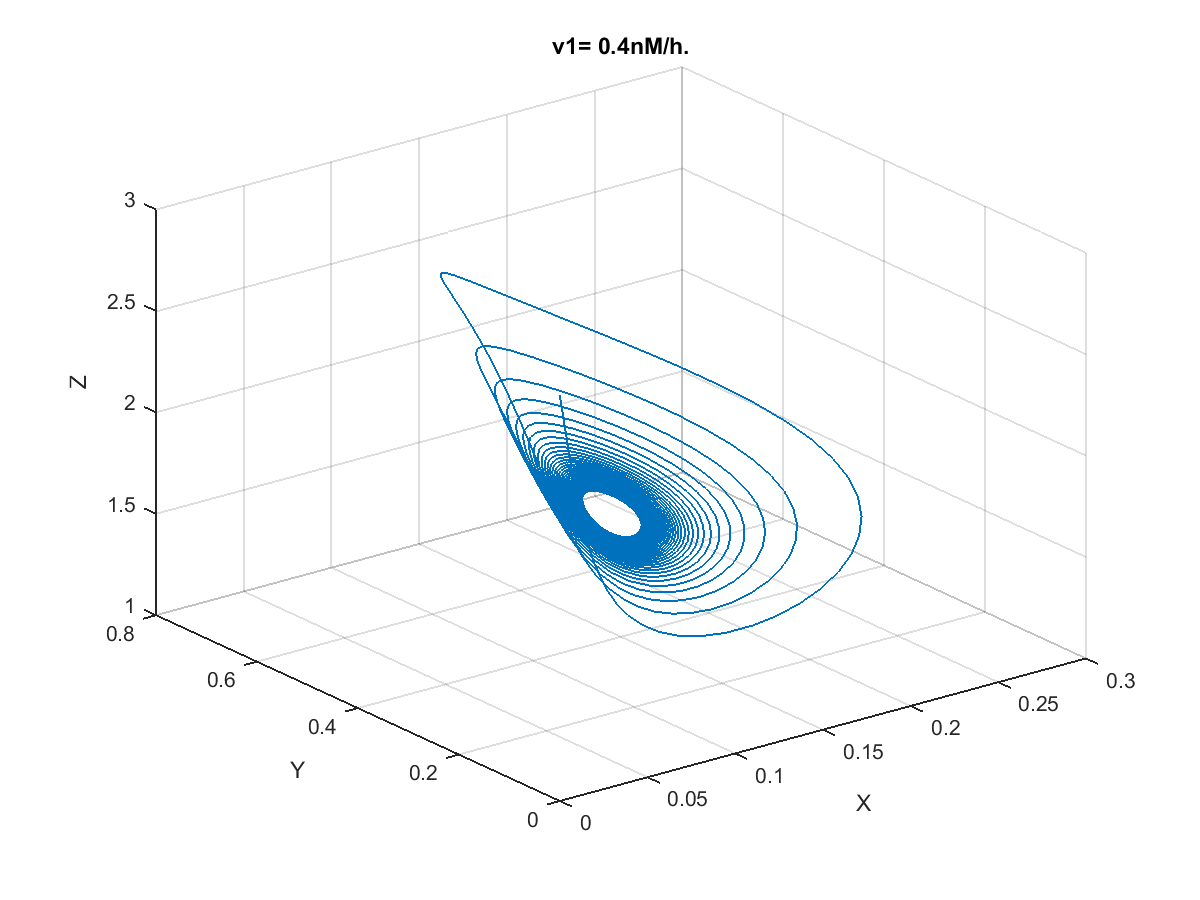
\includegraphics[width=\textwidth]{LotsofthesameA/A-AA4.png}
	    \caption{v1 = 4 nM/h}
	\end{subfigure}
	~
	\begin{subfigure}[b]{0.32\textwidth}
	    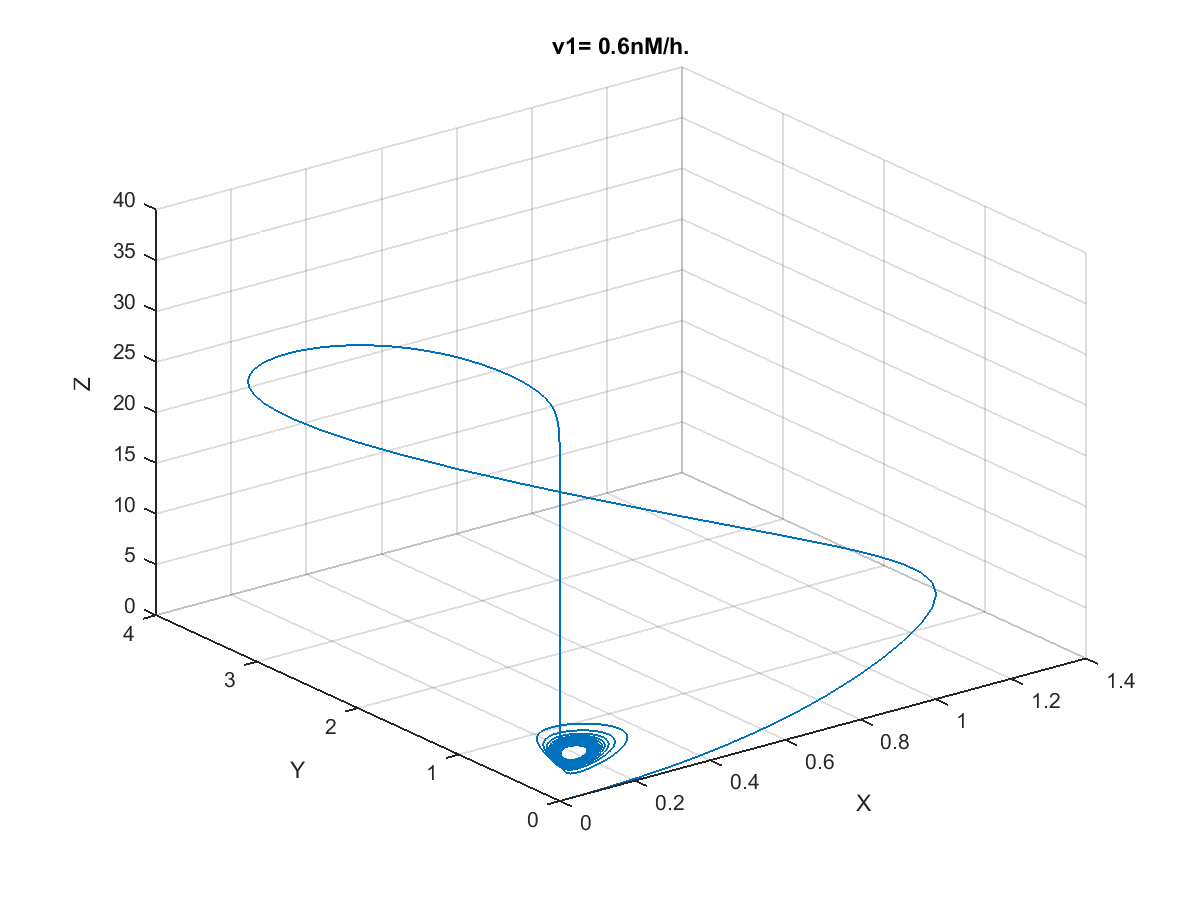
\includegraphics[width=\textwidth]{LotsofthesameA/A-AA6.png}
	    \caption{v1 = 6 nM/h}
	\end{subfigure}
	~ 
	\begin{subfigure}[b]{0.32\textwidth}
	    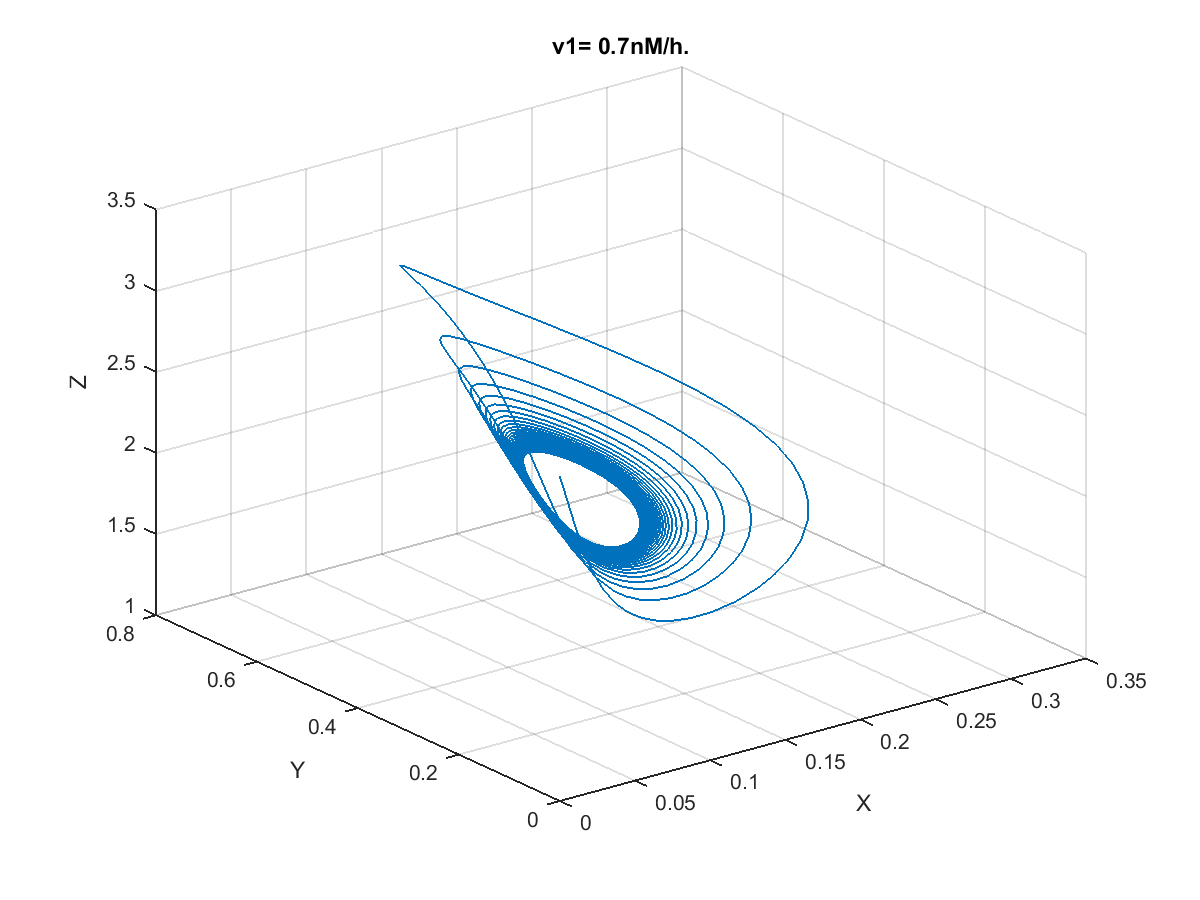
\includegraphics[width=\textwidth]{LotsofthesameA/A-AA7.png}
	    \caption{v1 = 8 nM/h}
	\end{subfigure}
	~
	\begin{subfigure}[b]{0.32\textwidth}
	    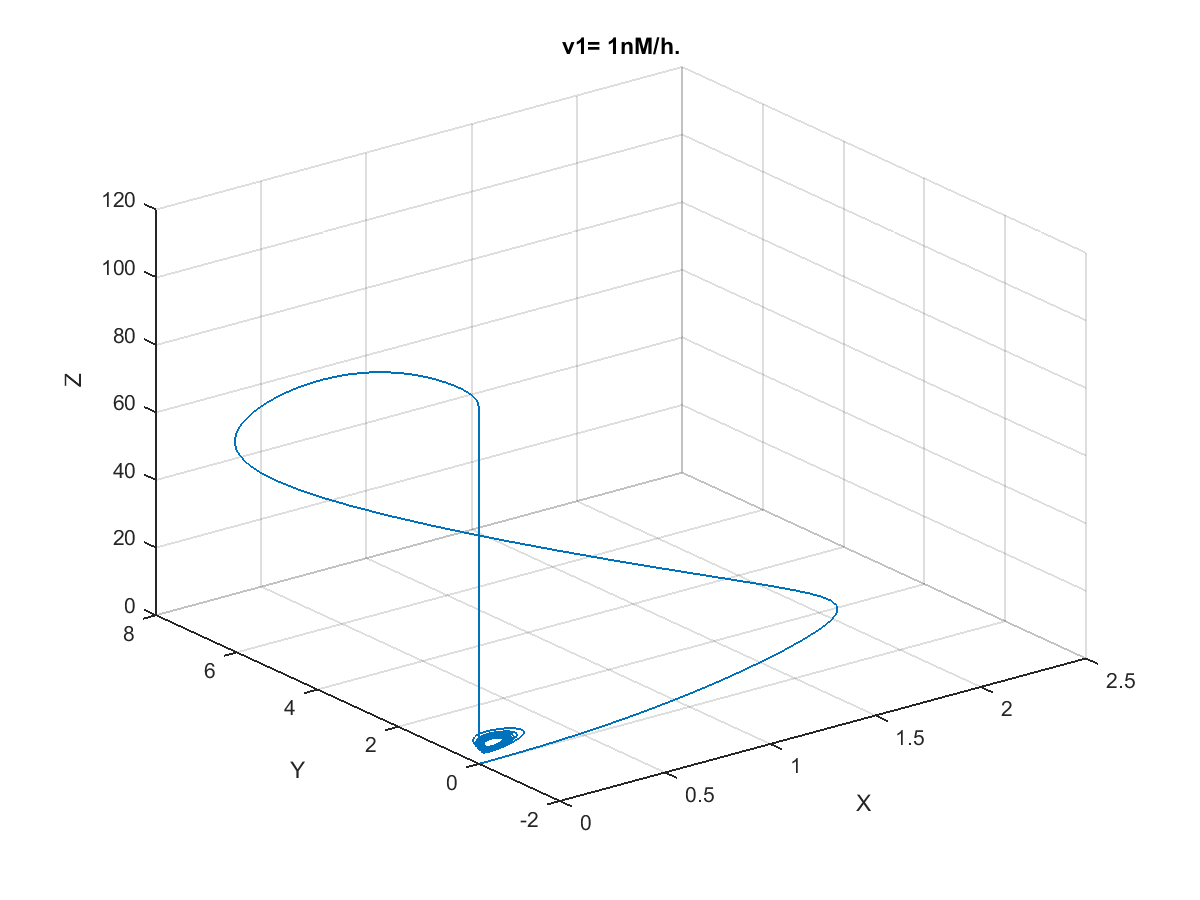
\includegraphics[width=\textwidth]{LotsofthesameA/A-AA10.png}
	    \caption{v1 = 10 nM/h}
	\end{subfigure}
	
	\caption{With nice initial conditions}
    \end{figure*}

    \begin{figure*}
    \centering
	\begin{subfigure}[b]{0.32\textwidth}
	    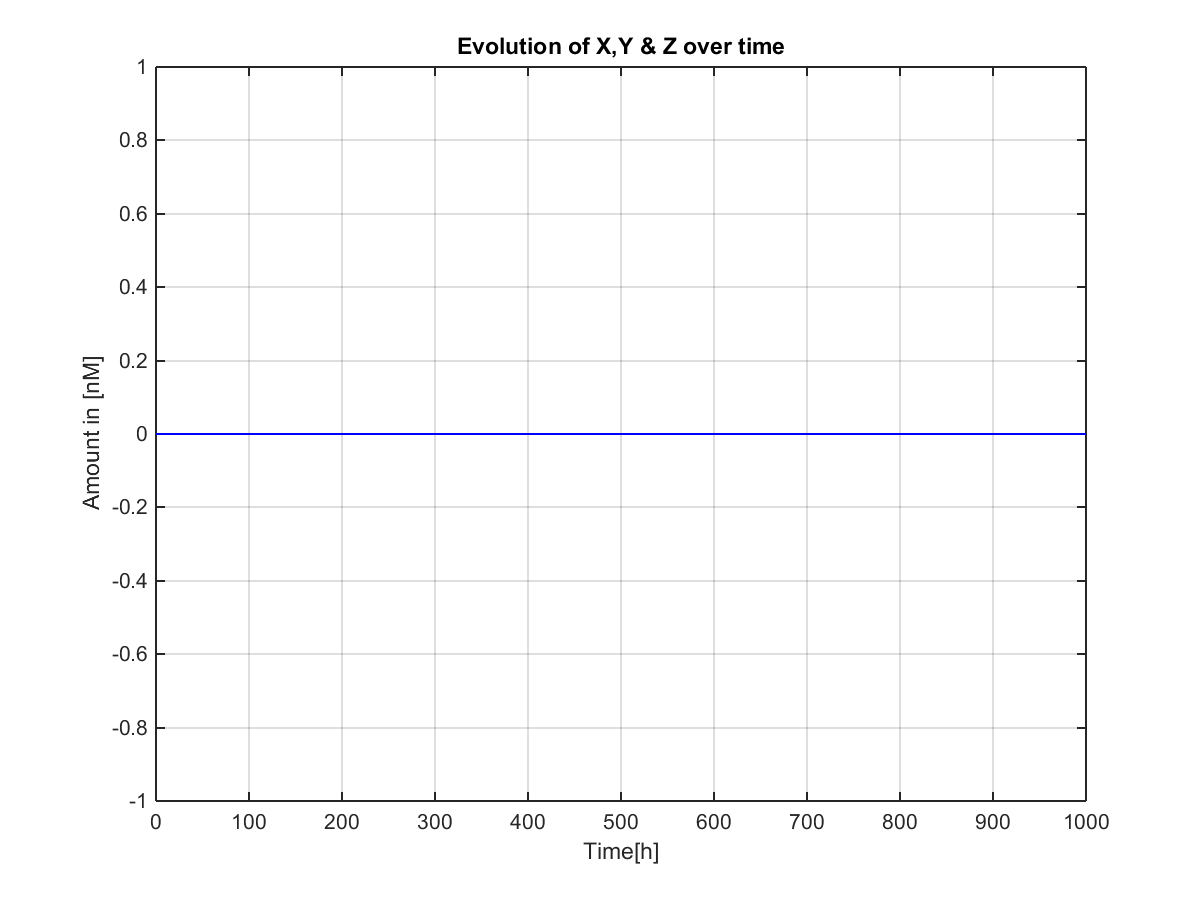
\includegraphics[width=\textwidth]{LotsofthesameA/A-A0.png}
	    \caption{v1 = 0 nM/h}
	\end{subfigure}
	~ 
	\begin{subfigure}[b]{0.32\textwidth}
	    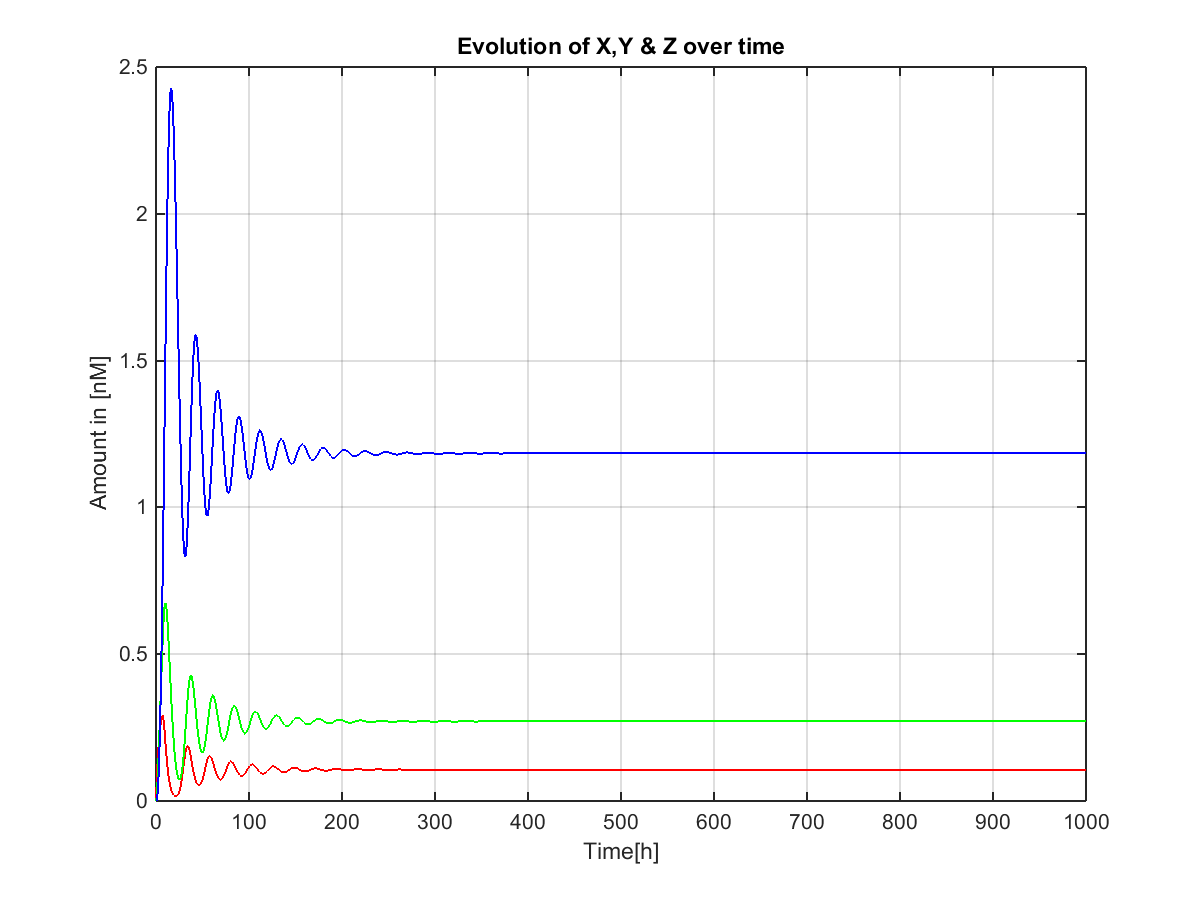
\includegraphics[width=\textwidth]{LotsofthesameA/A-A1.png}
	    \caption{v1 = 1 nM/h}
	\end{subfigure}
	~ 
	\begin{subfigure}[b]{0.32\textwidth}
	    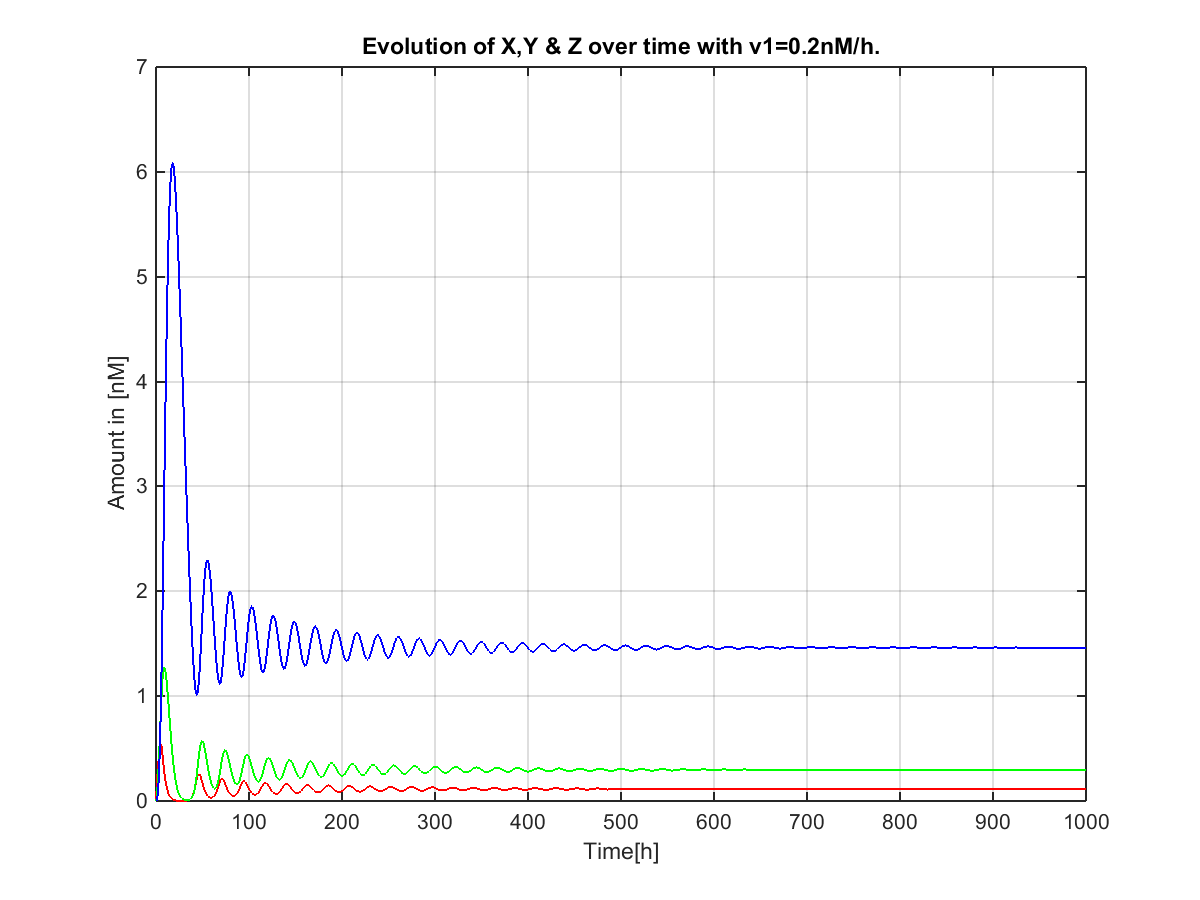
\includegraphics[width=\textwidth]{LotsofthesameA/A-A2.png}
	    \caption{v1 = 2 nM/h}
	\end{subfigure}
	 
	\begin{subfigure}[b]{0.32\textwidth}
	    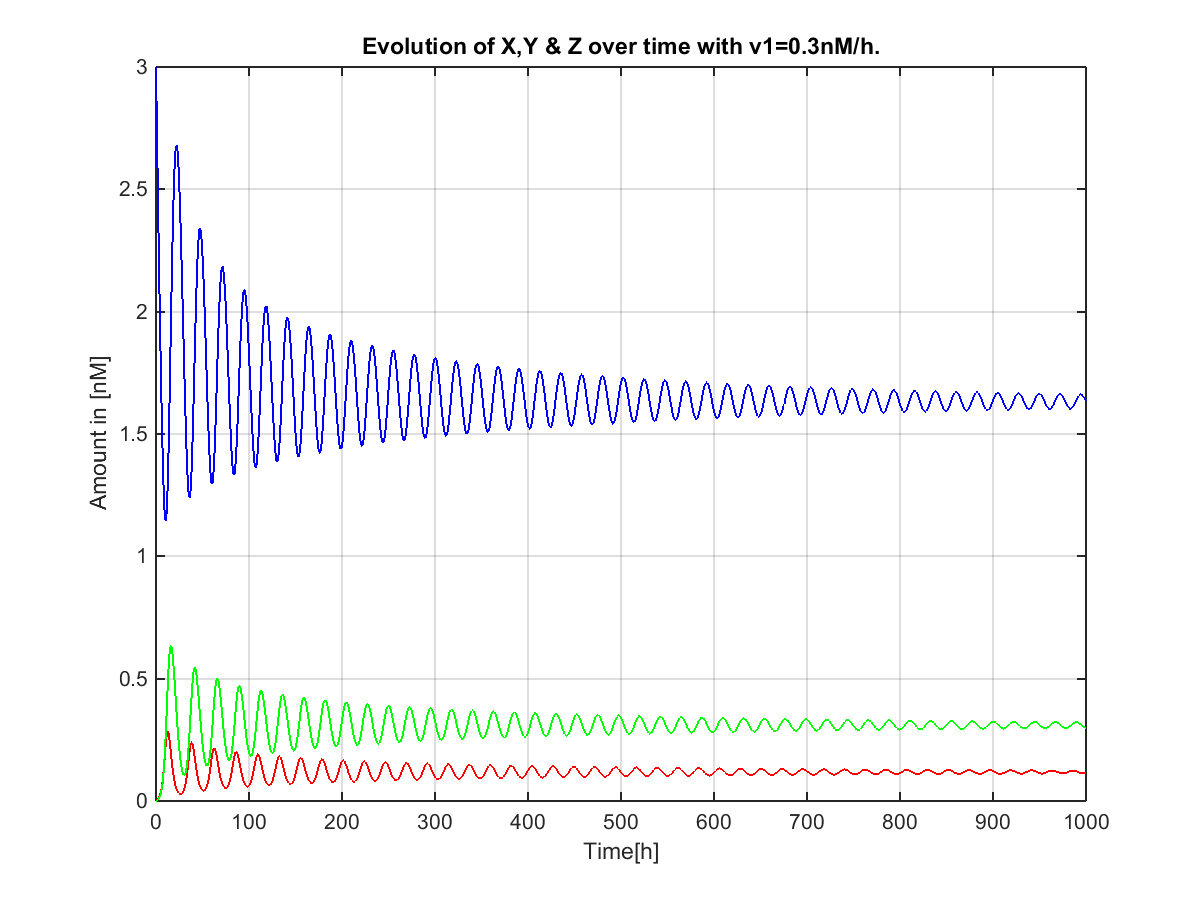
\includegraphics[width=\textwidth]{LotsofthesameA/A-A3.png}
	    \caption{v1 = 3 nM/h}
	\end{subfigure}
	~ 
	\begin{subfigure}[b]{0.32\textwidth}
	    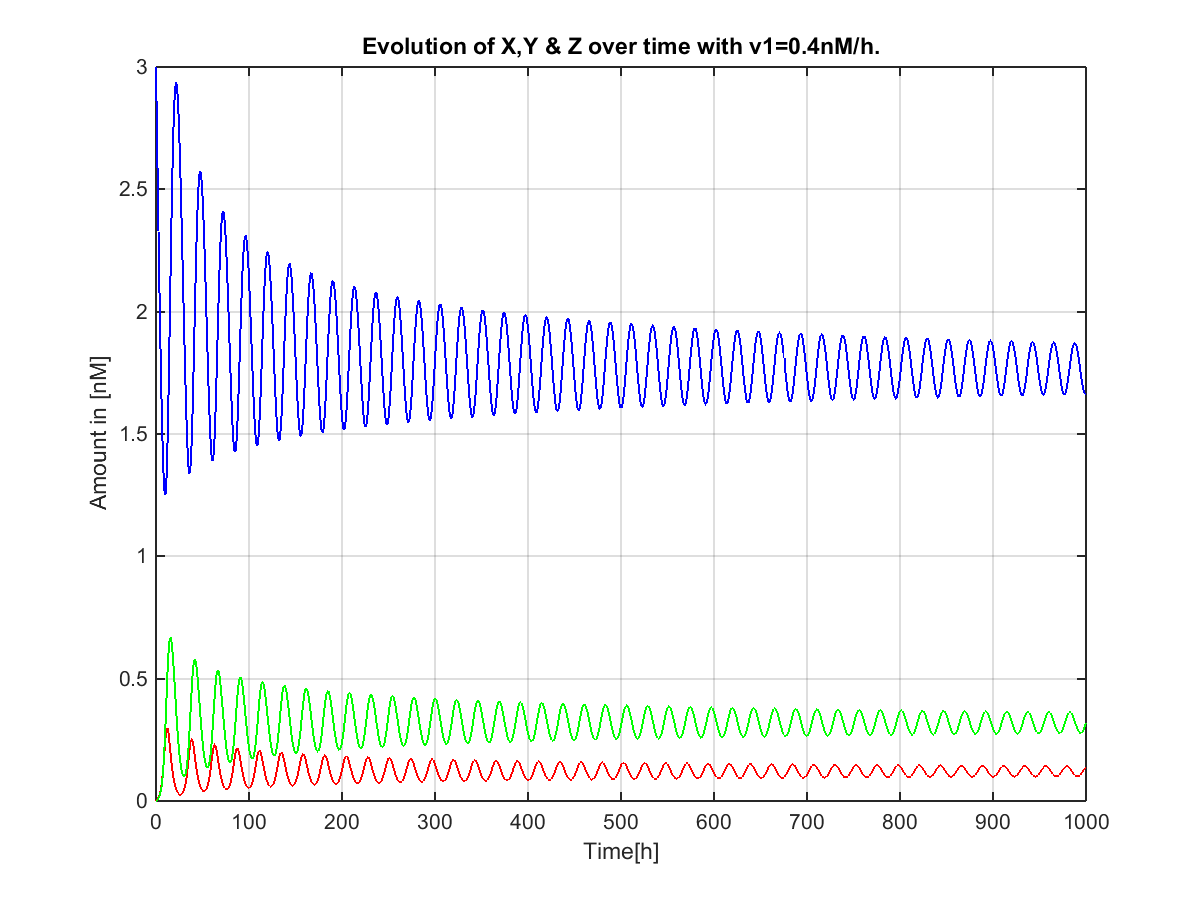
\includegraphics[width=\textwidth]{LotsofthesameA/A-A4.png}
	    \caption{v1 = 4 nM/h}
	\end{subfigure}
	~
	\begin{subfigure}[b]{0.32\textwidth}
	    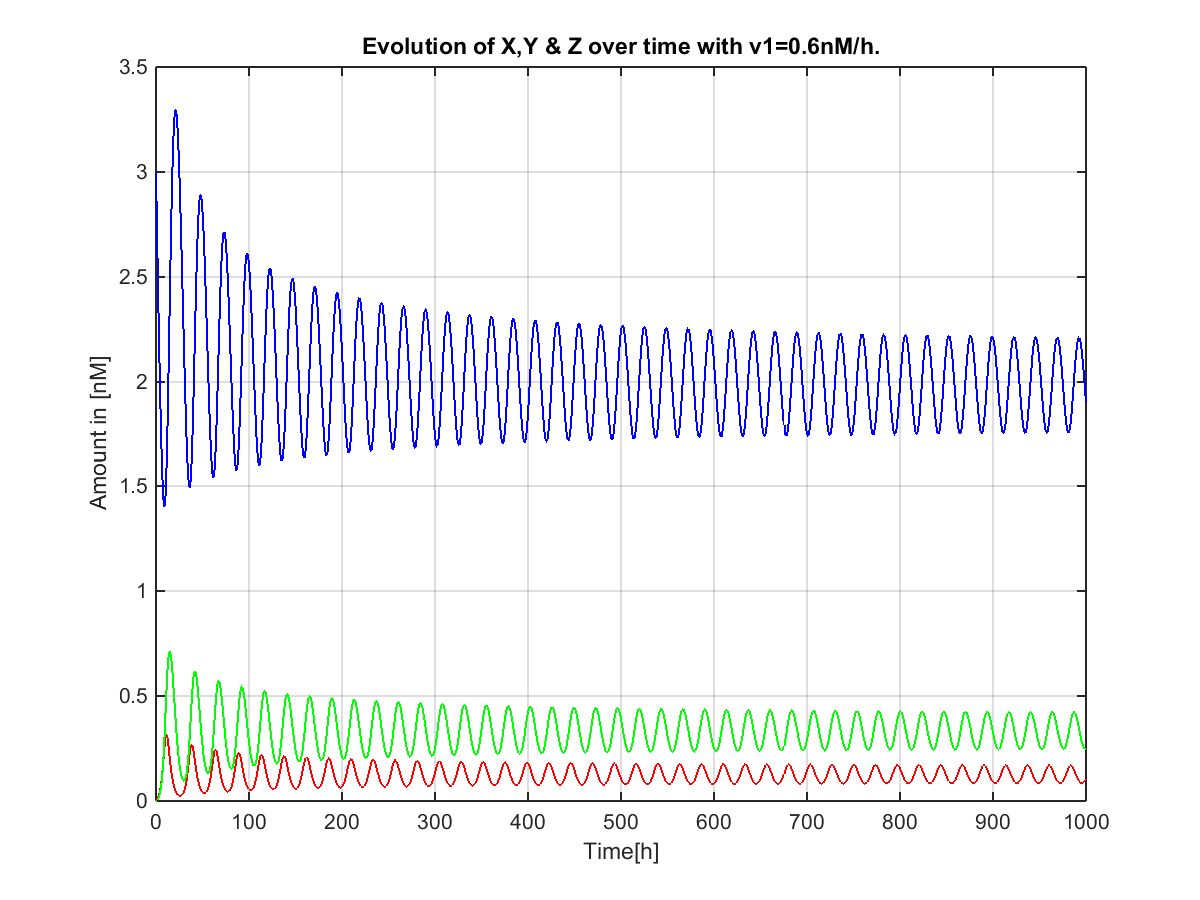
\includegraphics[width=\textwidth]{LotsofthesameA/A-A6.png}
	    \caption{v1 = 6 nM/h}
	\end{subfigure}
	~ 
	\begin{subfigure}[b]{0.32\textwidth}
	    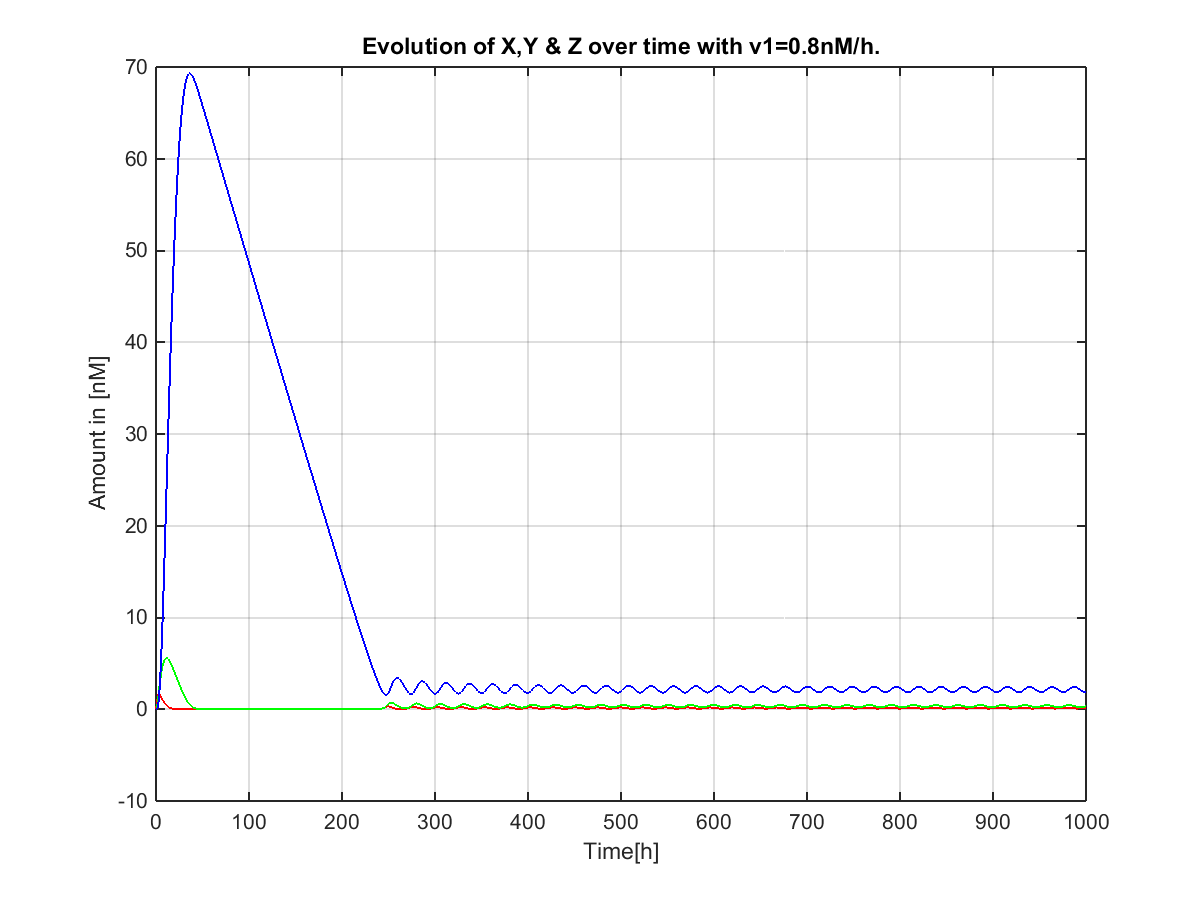
\includegraphics[width=\textwidth]{LotsofthesameA/A-A8.png}
	    \caption{v1 = 8 nM/h}
	\end{subfigure}
	~
	\begin{subfigure}[b]{0.32\textwidth}
	    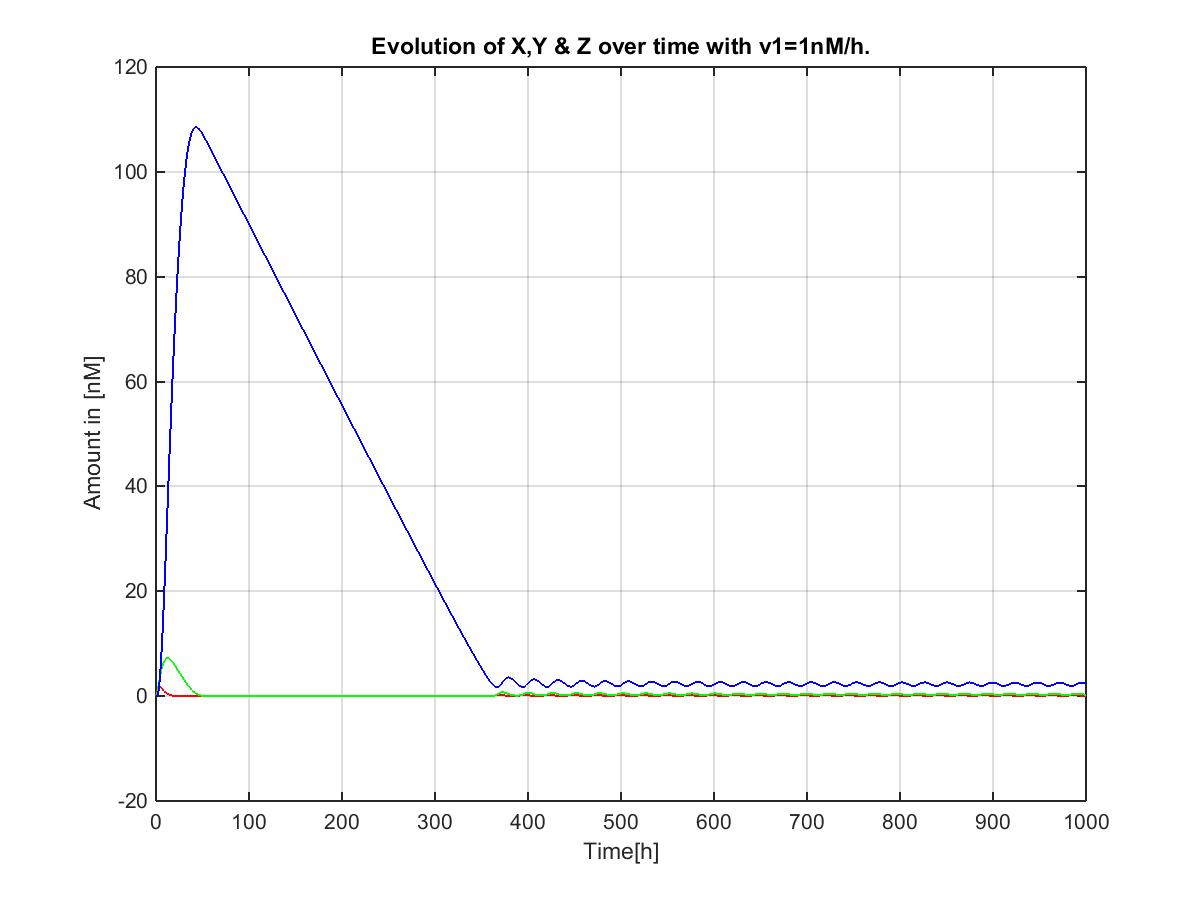
\includegraphics[width=\textwidth]{LotsofthesameA/A-A10.png}
	    \caption{v1 = 10 nM/h}
	\end{subfigure}

	\caption{With nice initial conditions}
    \end{figure*}

    \begin{figure*}
	\centering
	    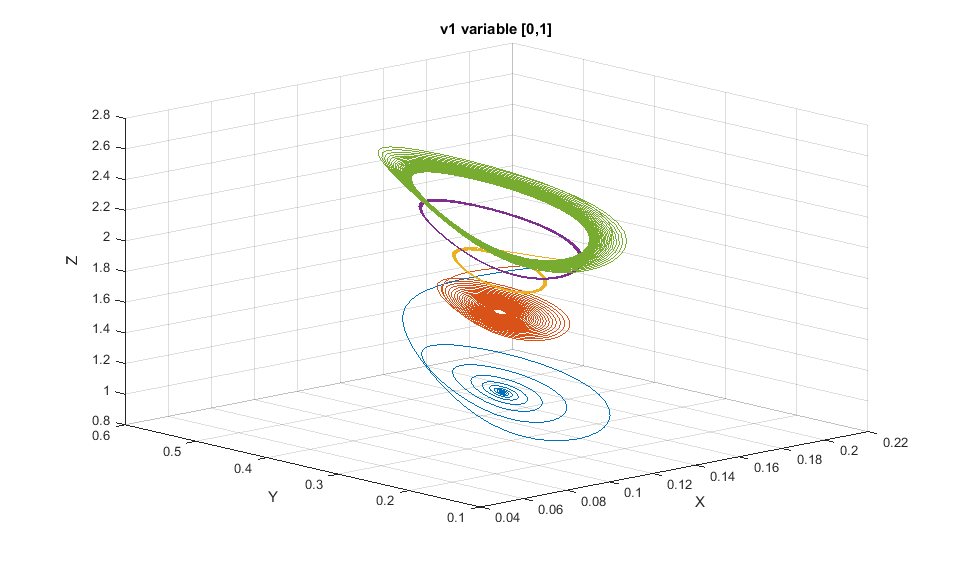
\includegraphics[width=0.5\textwidth]{A2.png}
	    \caption{v1 = 1/3/5/7/9 nM/h}
    \end{figure*}

    \begin{figure*}
	\centering
	    \begin{subfigure}[b]{0.45\textwidth}
		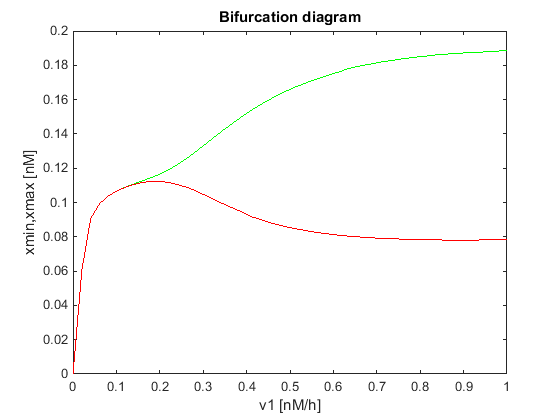
\includegraphics[width=\textwidth]{Bifurcation.png}
		\caption{v1 = 1/3/5/7/9 nM/h}
	    \end{subfigure}
	     ~ 
	    \begin{subfigure}[b]{0.45\textwidth}
		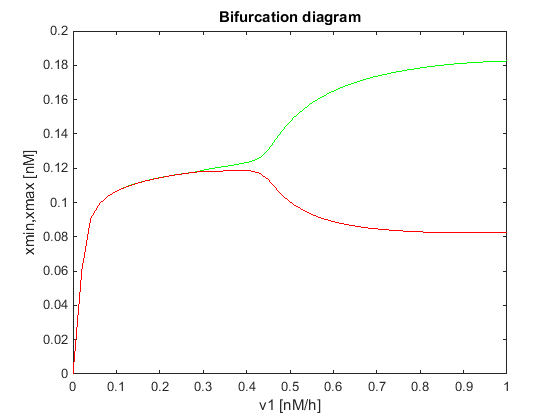
\includegraphics[width=\textwidth]{Bifurcation10000.png}
		\caption{v1 = 1/3/5/7/9 nM/h}
	    \end{subfigure}
    \end{figure*}

\end{document}
